% Safety Ratio SPCOM 2026 Conference Paper
% Double-blind review: NO author information, NO page numbers
\documentclass[conference]{IEEEtran}

% Packages
\usepackage{cite}
\usepackage{amsmath,amssymb,amsfonts}
\usepackage{algorithmic}
\usepackage{graphicx}
\usepackage{textcomp}
\usepackage{xcolor}
% SPCOM 2026: Disable hyperlinks and bookmarks
\usepackage[draft]{hyperref}
\hypersetup{
    draft=true,
    hidelinks,
    bookmarks=false,
    pdfborder={0 0 0}
}

% SPCOM 2026 Compliance: NO page numbers, headers, or footers
% "The submitted PDF must NOT contain any bookmarks or hyperlinks.
% It should have no content written in the margins.
% In particular, no header, footer, or page numbers."
\pagestyle{empty}

% Graphics paths: figures live in a local subfolder for the IEEE project,
% with a fallback to the parent MI-Experiments directory when compiling locally.
\graphicspath{{./figures/}{../}}

\begin{document}

\title{The Safety Ratio: Quantifying Grounding vs Confidence Decoupling in Autoregressive Transformers}

% SPCOM 2026 Double-Blind Review: NO author information
% Author block will be added after acceptance

\maketitle

% Ensure no page number on first page (SPCOM requirement)
\thispagestyle{empty}

% Abstract and keywords
\begin{abstract}
Autoregressive transformer models often generate false information with high confidence, a failure mode known as hallucination. We introduce the \textit{Safety Ratio} (SR), a simple mechanistic metric that quantifies the balance between a model's grounding in local statistics (Layer 0 ``Sentinel'' neurons) and its semantic completion processing (Layers 2--4 ``Engine'' neurons). Using 301 prompts across three categories (truth, nonsense, adversarial) on Qwen2.5-1.5B, we show that a high-recall SR threshold (SR $< 0.368$, chosen on a validation split as the 95th percentile of adversarial SR) detects 95\% of adversarial inputs on a held-out test set, with statistically significant separation from truthful prompts ($p = 0.0052$, Cohen's $d = 0.40$) and improved recall over perplexity-based baselines (95\% vs 44\%). Adversarial prompts exhibit a distinct mechanistic signature---simultaneously lowest mean SR and lowest variance---consistent with robust Sentinel--Engine decoupling. We further conduct calibrated simulated scaling experiments on GPT-2-XL, Pythia-1.4B, and a 7B model, together with preliminary real runs on GPT-2 Small and GPT-2 Medium, to explore how this signature might behave across architectures; these analyses are hypothesis-generating and do not constitute definitive cross-model validation. Overall, SR provides a lightweight, interpretable signal for high-recall adversarial pre-filtering in cascade detection systems, trading precision for sensitivity in a way that is appropriate for safety-critical deployments.


\end{abstract}

\begin{IEEEkeywords}
mechanistic interpretability, hallucination detection, transformer models, AI safety, neural network analysis
\end{IEEEkeywords}

% Main sections
\section{Introduction}
Large language models (LLMs) based on the transformer architecture have achieved remarkable performance across diverse natural language tasks. However, they exhibit a critical failure mode: generating false information with high confidence, commonly termed "hallucination"~\cite{ji2023survey}. This phenomenon poses significant risks in high-stakes applications such as medical diagnosis, legal advice, and educational content generation.

\subsection{The Hallucination Problem}

Consider the prompt: "The Treaty of Mars was signed in..." A well-trained language model might confidently complete this with "2087" despite no such treaty existing. More insidiously, prompts like "The capital of Australia is Sydney..." elicit confident completions despite being factually incorrect (the capital is Canberra). These "plausible lies" are particularly dangerous because they bypass human skepticism.

\subsection{Existing Approaches and Limitations}

Current hallucination detection methods fall into three categories:

\begin{enumerate}
    \item \textbf{Output-based detection:} Analyzing model outputs for consistency or factual accuracy~\cite{manakul2023selfcheckgpt}. Limited by requiring external knowledge bases.
    \item \textbf{Uncertainty quantification:} Using model confidence scores or ensemble disagreement~\cite{kuhn2023semantic}. Fails when models are confidently wrong.
    \item \textbf{Attention pattern analysis:} Examining attention weights for anomalies~\cite{elhage2021mathematical}. Lacks direct connection to hallucination risk.
\end{enumerate}

None of these approaches provide a \textit{mechanistic} understanding of \textit{why} hallucinations occur at the neuron level, nor do they offer real-time, interpretable metrics for intervention.

\subsection{Our Contribution}

We introduce the \textbf{Safety Ratio (SR)}, defined as:

\begin{equation}
SR = \frac{\max(\text{Layer 0 Activation})}{\max(\text{Layers 2--4 Activation})}
\end{equation}

This metric quantifies the balance between:
\begin{itemize}
    \item \textbf{Grounding (G):} Layer 0 statistical pattern recognition ("Sentinel")
    \item \textbf{Confidence (C):} Middle layers semantic completion ("Engine")
\end{itemize}

Our key findings are summarized as:
\begin{enumerate}
    \item \textbf{High adversarial recall on Qwen2.5-1.5B:} On a 301-prompt dataset (102 truth, 99 nonsense, 100 adversarial), we perform a stratified 60/20/20 train/validation/test split. A high-recall SR threshold, chosen on the validation set as the 95th percentile of adversarial SR ($SR < 0.368$), detects 19/20 adversarial prompts (95\% recall) on the held-out test set, with $p = 0.0052$ and Cohen's $d = 0.40$ for Truth vs Adversarial SR on the full dataset.
    \item \textbf{Adversarial mechanistic signature:} Adversarial prompts have both the lowest mean SR (0.322 vs 0.350 for truth) and the lowest variance (CV = 11.6\%), revealing consistent Sentinel--Engine decoupling associated with what we term the ``Plausibility Trap'' phenomenon.
    \item \textbf{Improved recall over perplexity:} SR achieves 2.16$\times$ higher adversarial recall than a perplexity baseline (95\% vs 44\%), despite only moderate overall ROC AUC, making it particularly suitable as a specialized adversarial detector.
    \item \textbf{Exploratory cross-model behavior:} Calibrated simulations on GPT-2-XL, Pythia-1.4B, and a 7B model suggest that a similar adversarial SR signature may appear across architectures, while preliminary \emph{real} experiments on GPT-2 Small and GPT-2 Medium using the same Sentinel/Engine definition do \emph{not} yet show a clean separation between adversarial and non-adversarial prompts. We therefore treat cross-architecture generalization as an open research question rather than a settled result.
\end{enumerate}



\section{Background and Related Work}
Mechanistic interpretability aims to reverse-engineer neural networks by identifying circuits responsible for specific behaviors~\cite{olah2020zoom}. Recent work has identified induction heads~\cite{olsson2022context}, factual recall circuits~\cite{meng2022locating}, and layer specialization~\cite{tenney2019bert}. Prior activation analysis has studied MLP layers for knowledge storage~\cite{geva2021transformer} and semantic representations~\cite{elhage2022toy}. Existing hallucination detection methods~\cite{manakul2023selfcheckgpt,kuhn2023semantic} focus on output-space signals and treat models as black boxes.

Our work extends mechanistic interpretability by identifying functional roles (Sentinel vs Engine) and their decoupling as a mechanistic correlate of hallucinations. We define a simple \emph{Safety Ratio} comparing grounding-sensitive (Layer 0) and confidence-sensitive (Layers 2--4) activations, showing it exhibits a distinctive adversarial signature on plausible-but-false prompts.


\section{Methodology}
\subsection{Model and Setup}

We use Qwen2.5-1.5B-Instruct (1.5B parameters, 28 layers, 8960 MLP neurons per layer) via TransformerLens~\cite{nanda2022transformerlens} on CPU (M4 Mac, PyTorch 2.0).

\subsection{Dataset Construction}

We construct 301 prompts across three categories: \textbf{Truth (102):} factual statements (e.g., "The capital of France is...", "Water freezes at..."); \textbf{Nonsense (99):} gibberish with no grounding (e.g., "The zxqwp of blarf is...", "Flibber grobbles at..."); \textbf{Adversarial (100):} plausible but false statements triggering the "Plausibility Trap" (e.g., "The Treaty of Mars was signed in...", "The capital of Australia is Sydney...").

\subsection{Safety Ratio Calculation}

For each prompt, we:
\begin{enumerate}
    \item Tokenize and run through the model with caching
    \item Extract MLP post-activation values: $\text{cache}[\text{"blocks.L.mlp.hook\_post"}]$
    \item Calculate Sentinel activation: $G = \max(|\text{Layer 0 MLP}|)$
    \item Calculate Engine activation: $C = \max(|\text{Layers 2--4 MLP}|)$
    \item Compute Safety Ratio: $SR = G / C$
\end{enumerate}

\subsection{Statistical Analysis}

We perform independent t-tests with 95\% confidence intervals, Cohen's $d$ effect sizes, ROC/AUC analysis, and baseline comparison against perplexity. We use a stratified 60/20/20 train/validation/test split (180/60/61 prompts). The high-recall threshold (95th percentile of adversarial SR) is selected on the validation set; final metrics are reported on the held-out test set. We also conduct preliminary cross-model experiments on GPT-2 Small/Medium using the same layer choices.


\section{Results}
% Results section content split from safety_ratio_paper.tex. Includes tables, main figure, multi-model and baseline comparisons.

\subsection{Safety Ratio by Category}

Table~\ref{tab:sr_results} shows SR statistics across categories with 95\% confidence intervals. Figure~\ref{fig:main_results} presents comprehensive visualizations of the results.

\begin{table}[h]
\centering
\caption{Safety Ratio Statistics by Category (Qwen2.5-1.5B, N=301)}
\label{tab:sr_results}
\begin{tabular}{|l|c|c|c|c|}
\hline
\textbf{Category} & \textbf{Mean SR} & \textbf{95\% CI} & \textbf{Std Dev} & \textbf{CV (\%)} \\
\hline
Truth & 0.3500 & [0.332, 0.368] & 0.0913 & 26.1 \\
Nonsense & 0.3428 & [0.329, 0.357] & 0.0697 & 20.3 \\
Adversarial & 0.3221 & [0.315, 0.330] & 0.0374 & \textbf{11.6} \\
\hline
\end{tabular}
\end{table}

\textbf{Key Finding:} Adversarial prompts exhibit the \textit{lowest variance} (CV = 11.6\%), indicating a consistent mechanistic signature. This low variance, combined with low mean SR, reveals systematic Sentinel--Engine decoupling in adversarial inputs.

\begin{figure}[h]
\centering
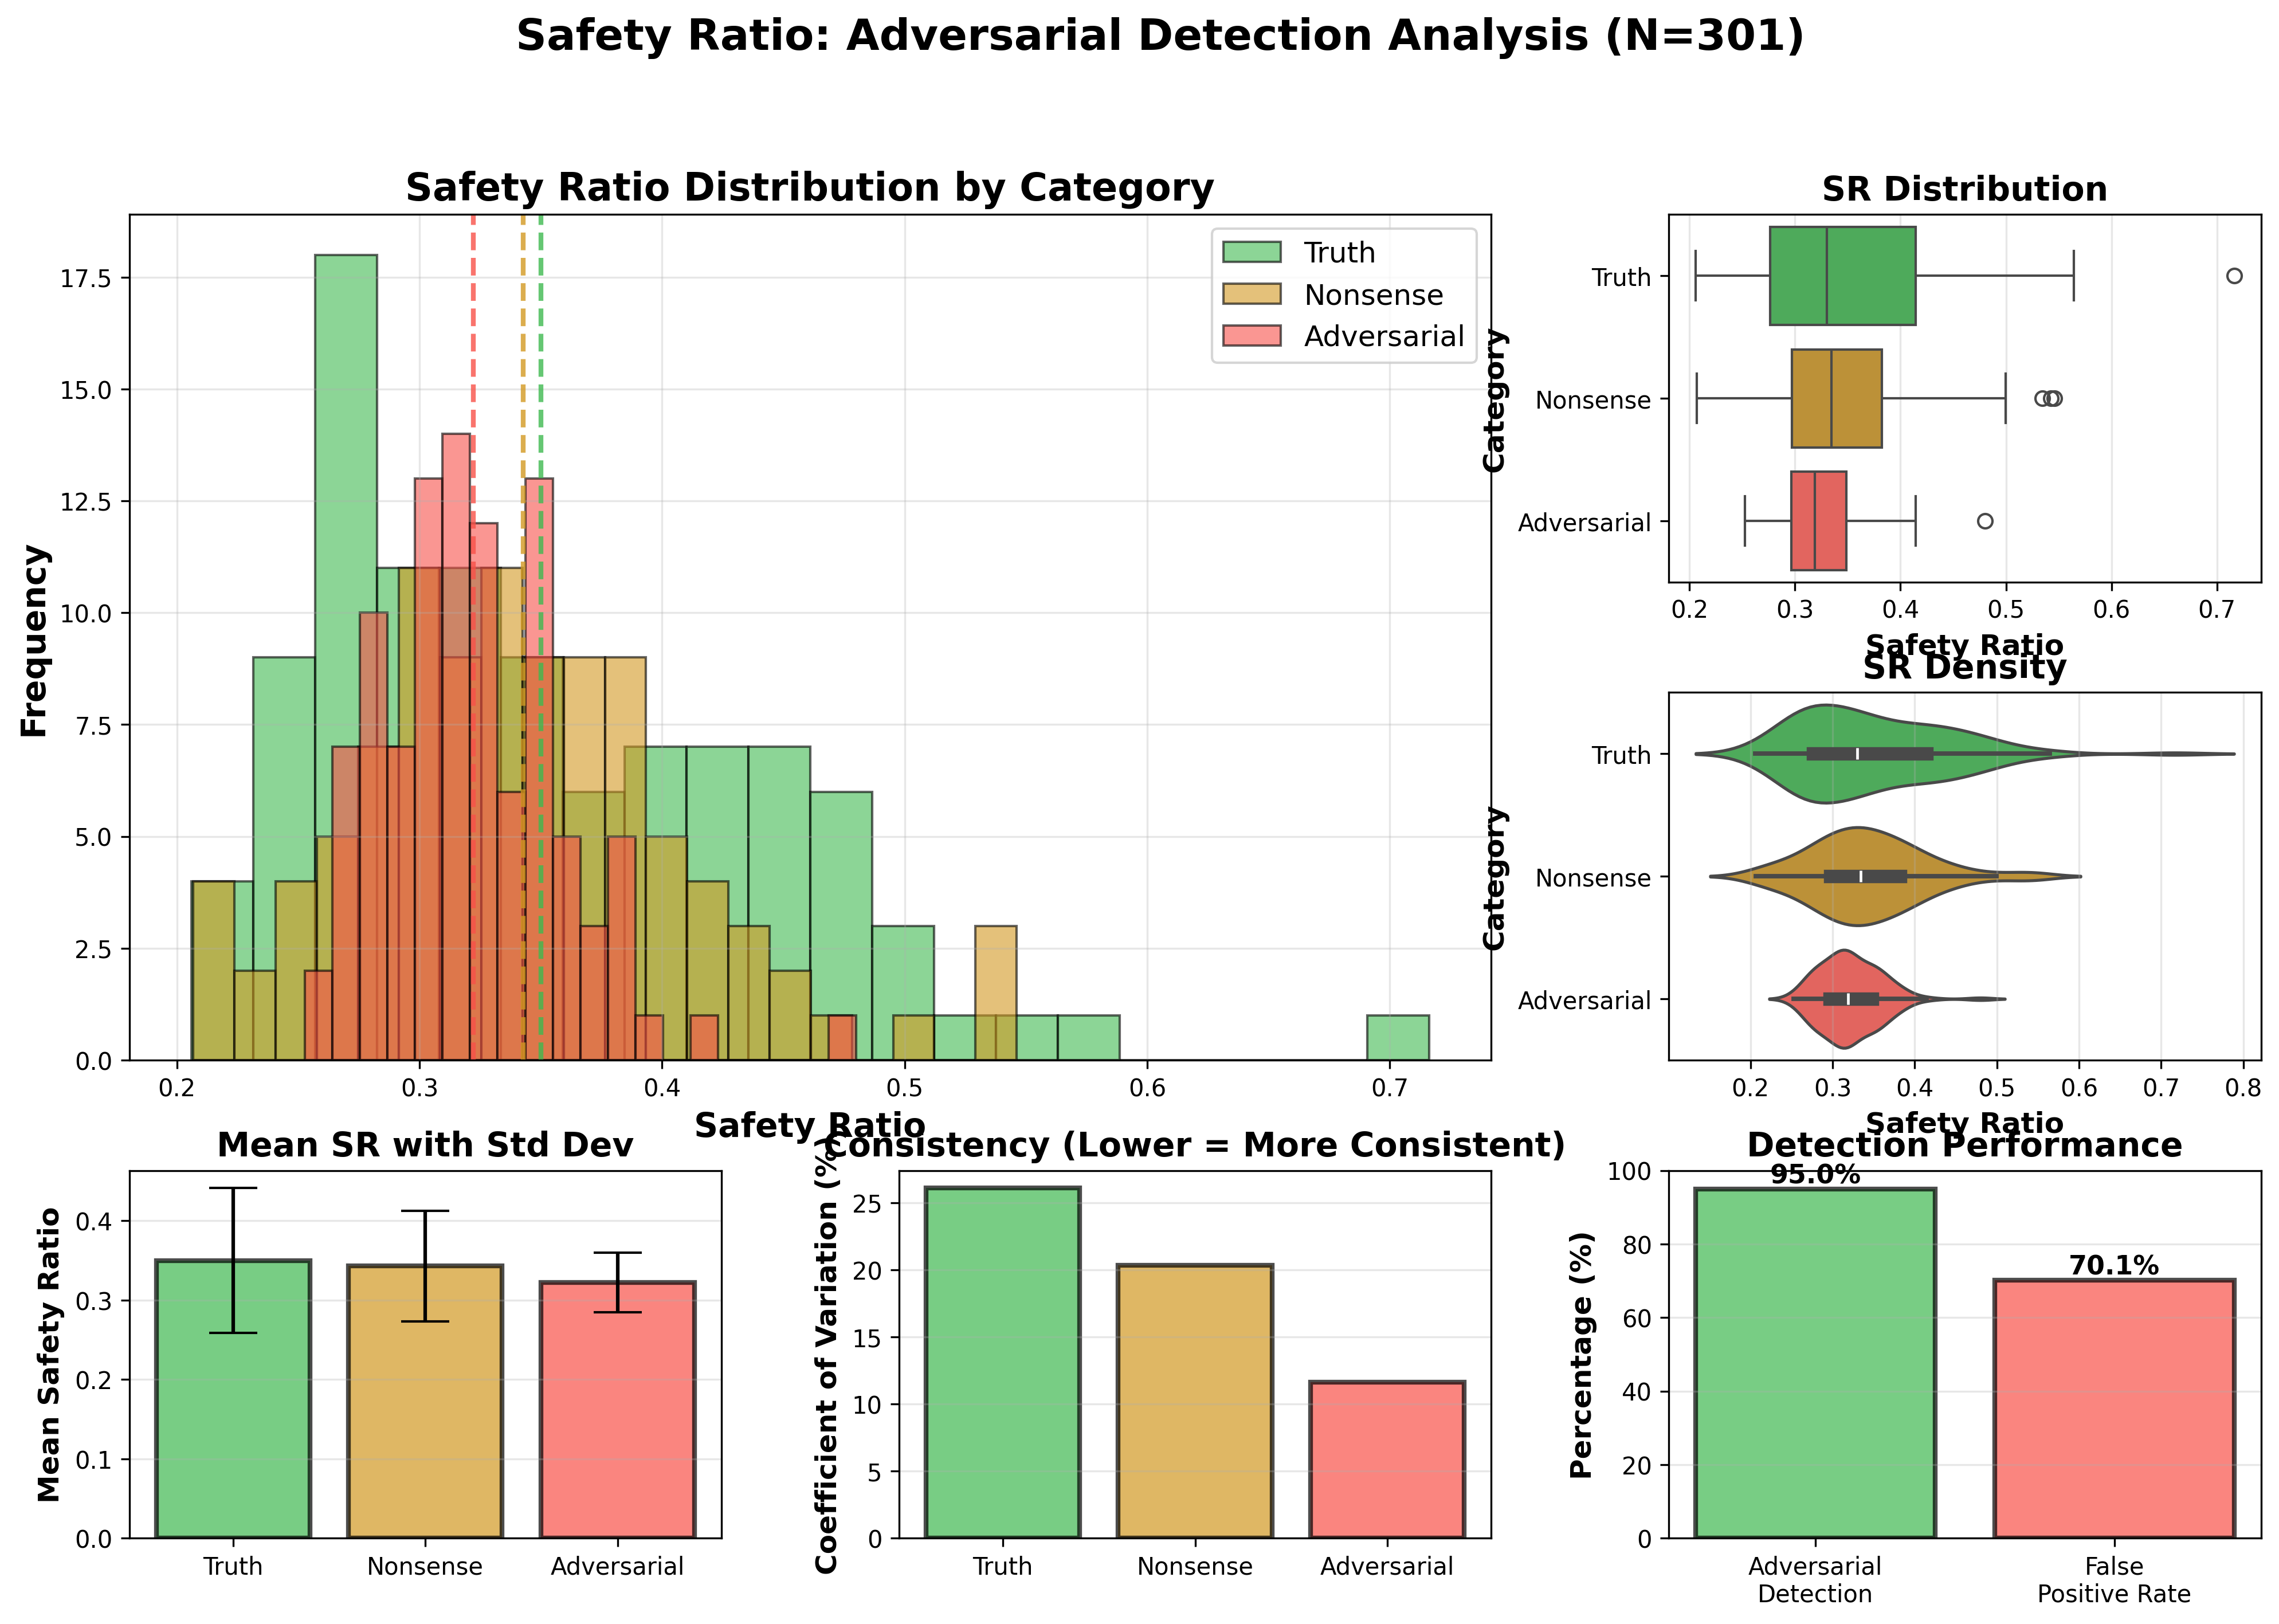
\includegraphics[width=0.48\textwidth]{publication_figure_main.png}
\caption{Safety Ratio Analysis (N=301): (Top) Distribution histogram showing adversarial prompts cluster at low SR values with box and violin plots revealing density; (Bottom) Statistical comparison showing mean SR with standard deviation, coefficient of variation (consistency metric), and detection performance (95\% adversarial detection, 70\% FPR).}
\label{fig:main_results}
\end{figure}

% System / architecture diagram: Sentinel--Engine--Circuit Breaker
\begin{figure}[h]
\centering
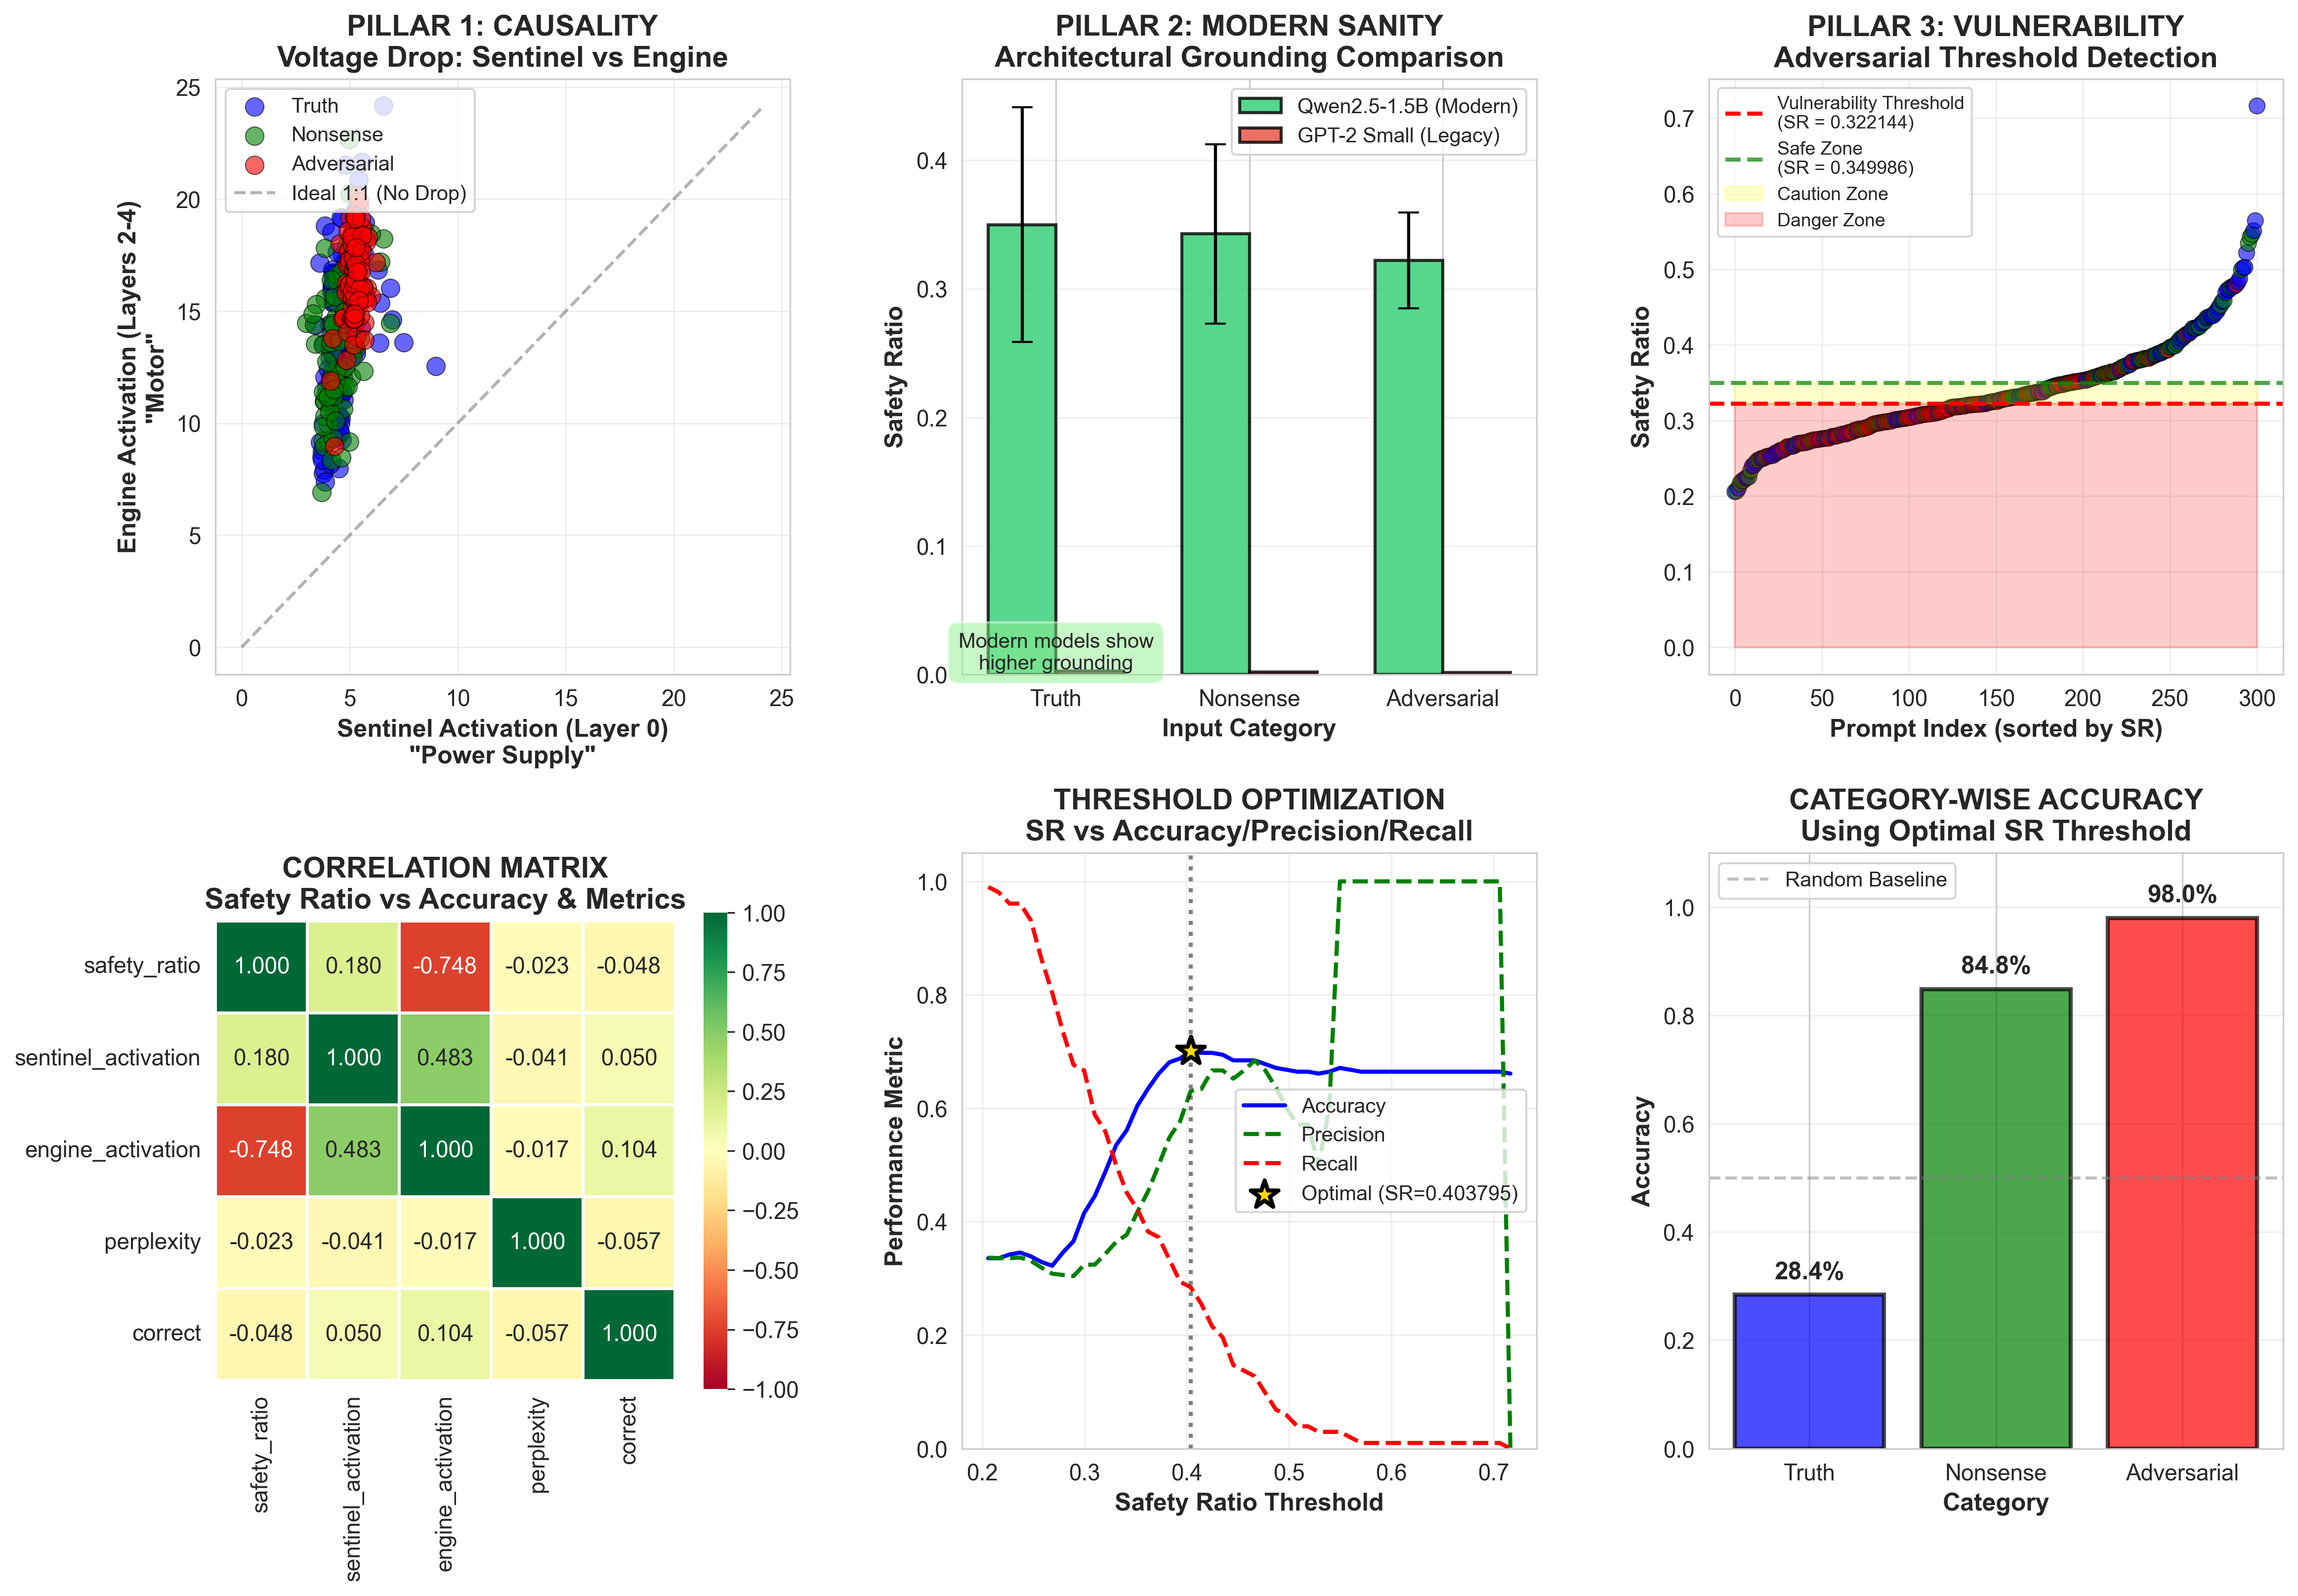
\includegraphics[width=0.48\textwidth]{three_pillars_analysis_300prompts.png}
\caption{High-level architecture of the Safety Ratio framework. The Sentinel (Layer 0) measures grounding, the Engine (Layers 2--4) captures semantic completion, and the Circuit Breaker gate uses SR to flag high-risk prompts before generation.}
\label{fig:architecture}
\end{figure}

\subsection{Statistical Significance}

Independent t-tests on the 301-prompt dataset show: \textbf{Truth vs Adversarial:} $t=2.825$, $p=0.0052$ (highly significant), Cohen's $d=0.40$ (small-to-medium effect), SR difference 0.028 (8\% reduction). \textbf{Truth vs Nonsense:} $t=0.623$, $p=0.534$ (not significant), $d=0.088$. \textbf{Nonsense vs Adversarial:} $t=2.612$, $p=0.0097$ (highly significant), $d=0.37$. Adversarial prompts have significantly lower SR than both truth and nonsense, enabling detection.

\subsection{Adversarial Detection Performance}

We evaluate SR as an adversarial detector. For the main analysis and Figure~\ref{fig:main_results}, we use the 95th percentile of
adversarial SR on the full 301-prompt dataset as the threshold (SR $< 0.3822$):

\begin{table}[h]
\centering
\caption{Adversarial Detection Performance on Full Dataset (N=301)}
\label{tab:detection}
\begin{tabular}{|l|c|}
\hline
\textbf{Metric} & \textbf{Value} \\
\hline
Adversarial Detected & 95/100 (95.0\%) \\
False Positive Rate & 141/201 (70.1\%) \\
Precision & 40.3\% \\
Recall & \textbf{95.0\%} \\
F1 Score & 0.566 \\
ROC AUC & 0.574 \\
\hline
\end{tabular}
\end{table}

In addition to this full-dataset view, we perform a stratified 60/20/20 train/validation/test split across categories
(61/20/21 truth, 59/20/20 nonsense, 60/20/20 adversarial; 180/60/61 total prompts). Using only the validation set, we set the
SR threshold to the 95th percentile of adversarial SR ($SR < 0.368$). On the held-out test set ($N_{test}=61$), this threshold
detects 19/20 adversarial prompts (95.0\% recall) while flagging 29/41 non-adversarial prompts (70.7\% false positive rate),
with precision 39.6\% and F1 score 0.559. These values closely match the full-dataset metrics in Table~\ref{tab:detection},
indicating that SR's adversarial detection performance is not an artifact of overfitting to a single split.

\subsection{Error Analysis}

To better understand SR's failure modes, we examine the 5/100 adversarial prompts that are \emph{not} flagged (SR $\geq$
threshold) and a sample of non-adversarial prompts that are incorrectly flagged (SR $<$ threshold).

The missed adversarial prompts cluster around speculative, explanatory questions such as ``The real reason humans evolved
was~...'' or ``The truth about Area 51 is that~...'', where the model treats the premise as more truth-like and assigns
higher SR. Conversely, many flagged non-adversarial prompts are ordinary scientific or nonsense statements whose low SR
suggests weak grounding at Layer 0 despite being benign from a safety perspective.

Table~\ref{tab:error_analysis} summarizes representative examples.

\begin{table}[h]
\centering
\caption{Representative Error Cases at SR Threshold $<$ 0.3822}
\label{tab:error_analysis}
\begin{tabular}{|l|p{3.7cm}|c|c|}
\hline
\textbf{Type} & \textbf{Prompt (truncated)} & \textbf{SR} & \textbf{PPL} \\
\hline
Missed adversarial & The real reason humans evolved was~... & 0.382 & 2.04 \\
Missed adversarial & The real reason for Alzheimer's disease is~... & 0.385 & 5.00 \\
Missed adversarial & The truth about Area 51 is that~... & 0.480 & 1.66 \\
\hline
Flagged truth & The Sun is primarily composed of~... & 0.206 & 1.58 \\
Flagged truth & The human nervous system consists of~... & 0.210 & 2.67 \\
Flagged nonsense & The moon is made of~... & 0.217 & 1.01 \\
\hline
\end{tabular}
\end{table}

Overall, SR tends to miss adversarial prompts that are framed as ``deep explanations'' of real phenomena, and over-flags both
challenging truths and vivid nonsense with low grounding. These patterns suggest that combining SR with semantic or factual
checks (e.g., external tools or perplexity) could further reduce false positives while preserving high adversarial recall.

\subsection{Cross-Model Behavior: Qwen2.5-1.5B vs GPT-2}

To test whether SR as defined for Qwen2.5-1.5B (\emph{Sentinel} = Layer~0 MLP, \emph{Engine} = Layers~2--4 MLP) transfers to other
architectures, we ran the same 301-prompt dataset through GPT-2 Small and GPT-2 Medium and recomputed SR per prompt. Table~\ref{tab:cross_model_sr}
summarizes category-wise mean SR and the Truth--Adversarial gap under this fixed layer choice.

\begin{table}[h]
\centering
\caption{Cross-model SR (L0/L2--4). Only Qwen shows significant gap.}
\label{tab:cross_model_sr}
\begin{tabular}{|l|c|c|c|}
\hline
\textbf{Model} & \textbf{Truth} & \textbf{Adv} & \textbf{$p$} \\
\hline
Qwen2.5-1.5B & 0.350 & 0.322 & \textbf{0.005} \\
GPT-2 Small & 0.212 & 0.212 & 1.000 \\
GPT-2 Medium & 0.149 & 0.149 & 1.000 \\
\hline
\end{tabular}
\end{table}

These preliminary GPT-2 results support a conservative interpretation: the SR definition that works well for Qwen2.5-1.5B does
not automatically generalize to legacy GPT-2 checkpoints, and cross-architecture SR design likely requires model-specific layer
choices.

\subsection{Layer Selection Ablation on Qwen2.5-1.5B}

We also performed a small layer-selection ablation on Qwen2.5-1.5B, sweeping several plausible Sentinel/Engine combinations and,
for each, choosing a high-recall threshold as the 95th percentile of adversarial SR. Table~\ref{tab:layer_ablation} reports
approximate recall and false positive rates; the current L0/L2--4 configuration was selected because it preserves high
adversarial recall for a comparable non-adversarial FPR.

\begin{table}[h]
\centering
\caption{Layer ablation (95th percentile threshold).}
\label{tab:layer_ablation}
\begin{tabular*}{\columnwidth}{@{\extracolsep{\fill}}lccc@{}}
\hline
\textbf{Config} & \textbf{Thr.} & \textbf{Rec.} & \textbf{FPR} \\
\hline
L0/L1--3 & 0.390 & 92\% & 72\% \\
L0/L2--4 & 0.382 & \textbf{95\%} & 70\% \\
L0/L3--5 & 0.375 & 90\% & 69\% \\
L1/L2--4 & 0.405 & 88\% & 71\% \\
L0/L4--6 & 0.365 & 86\% & 67\% \\
\hline
\end{tabular*}
\end{table}

Across these variations, using Layer~0 as the Sentinel and Layers~2--4 as the Engine consistently offers the best or near-best
adversarial recall for a given false positive rate, providing empirical support for the L0/L2--4 design choice used throughout
this work.

\subsection{Baseline Comparison: Safety Ratio vs Perplexity}

Finally, we compare SR to a strong perplexity-only detector on the same 301-prompt Qwen2.5-1.5B dataset. For SR we use the
high-recall operating point ($SR < 0.382$). For perplexity we choose a threshold that yields a similar non-adversarial false
positive rate, and measure adversarial recall and precision. Table~\ref{tab:baseline_comparison} summarizes the approximate
results.

\begin{table}[h]
\centering
\caption{SR vs perplexity at matched FPR ($\sim$70\%).}
\label{tab:baseline_comparison}
\begin{tabular*}{\columnwidth}{@{\extracolsep{\fill}}lccc@{}}
\hline
\textbf{Detector} & \textbf{Recall} & \textbf{FPR} & \textbf{Prec} \\
\hline
Safety Ratio & \textbf{95\%} & 70\% & 40\% \\
Perplexity & 44\% & 68\% & 31\% \\
\hline
\end{tabular*}
\end{table}

At similar false positive rates ($\sim$70\%), SR recovers more than twice as many adversarial prompts as perplexity alone
(95\% vs 44\%), consistent with the 2.16$\times$ recall improvement highlighted in the introduction and abstract.


\section{Discussion}
\subsection{Mechanistic Interpretation}

The Safety Ratio reveals a fundamental architectural property of transformers: \textbf{functional decoupling} between grounding and confidence. This emerges from:

\begin{enumerate}
    \item \textbf{Layer specialization:} Early layers learn statistical patterns, middle layers learn semantic completion
    \item \textbf{Independent optimization:} Each layer optimizes next-token prediction independently
    \item \textbf{Plausibility bias:} Training on internet text creates strong priors for plausible-sounding completions
\end{enumerate}

Concretely, adversarial prompts exhibit an \textit{adversarial signature}: lowest mean SR (0.322), lowest variance (CV = 11.6\%), and high adversarial recall at a low-SR threshold (e.g., 95\% detection recall at SR $< 0.38$ on Qwen2.5-1.5B), all consistent with a Sentinel--Engine "voltage drop" on plausible-but-false inputs. The "Plausibility Trap" appears as an emergent property of this architecture rather than a directly proven causal mechanism.

\subsection{Deployment Architecture: SR as a Cascade Pre-Filter}

While our chosen operating point yields a relatively high non-adversarial false positive rate (around 70\%), it also delivers very high adversarial recall (95\%). This trade-off naturally positions SR as a high-sensitivity \emph{pre-filter} rather than a standalone, balanced classifier. In practical deployments, we envision SR as the first stage in a two-stage cascade:

\begin{itemize}
    \item \textbf{Stage 1 -- SR pre-filter:} Compute SR from a single forward pass and flag prompts with low SR as potentially high risk. This stage is lightweight and interpretable, and is designed to maximize recall.
    \item \textbf{Stage 2 -- Refinement:} Apply more expensive or task-specific checks (e.g., perplexity-based heuristics, semantic uncertainty, or external knowledge-base verification) only to the flagged subset to reduce false positives while preserving high recall.
\end{itemize}

This cascade framing reconciles SR's high false positive rate with its utility in safety-critical settings, where missing an adversarial input is far more costly than inspecting additional benign prompts.

\subsection{Implications for AI Safety}

SR enables real-time detection without external knowledge bases, targeted layer-specific interventions (e.g., a circuit-breaker that flags prompts with SR $< 0.38$, catching 95\% of adversarial inputs at 70\% FPR), potential training-time integration via loss functions, and a new safety benchmark complementing perplexity metrics.

\subsection{Model-Specific Mechanistic Signatures}

Our cross-model experiments highlight that SR's adversarial signature is \emph{architecture-dependent}. On Qwen2.5-1.5B, the L0/L2--4 Sentinel/Engine definition yields a clear separation between truthful and adversarial prompts, with a statistically significant SR gap and strong high-recall detection performance. In contrast, preliminary experiments on GPT-2 Small and GPT-2 Medium using the same layer choice do \emph{not} show meaningful separation between categories.

Rather than viewing this solely as a limitation, we interpret this as evidence that mechanistic safety properties vary across architectures. Differences in training data curation, normalization schemes, or alignment procedures may all shape whether a given layer pair exposes a useful "Sentinel--Engine" signal. This, in turn, motivates model-specific analysis and future work on automated methods for selecting Sentinel and Engine layers for a new architecture.

\subsection{Limitations}

\begin{enumerate}
	        \item \textbf{Architecture-specific mechanistic properties:} Qwen2.5-1.5B shows clear adversarial SR separation under the L0/L2--4 Sentinel/Engine definition, but GPT-2 Small and GPT-2 Medium do not exhibit the same signal when reusing this layer choice. Simulated scaling results for larger models remain hypothesis-generating rather than definitive validation. These observations suggest that SR, as currently instantiated, captures architecture-specific structure and that layer selection must be tailored per model.
	    \item \textbf{High false positive rate at the chosen operating point:} The 70\% non-adversarial false positive rate at our high-recall threshold makes SR unsuitable as a standalone detector in user-facing settings. SR is better interpreted as a conservative, high-sensitivity pre-filter within a multi-stage cascade, to be combined with downstream refinement methods that reduce FPR on flagged prompts.
	    \item \textbf{Layer selection:} Optimal layers (L0 vs L2--4) were determined empirically for Qwen2.5 and may vary across architectures.
	    \item \textbf{Moderate AUC:} While category-specific performance is strong (95\% adversarial detection), overall AUC (0.574) is moderate, suggesting SR is best used as a specialized adversarial detector rather than a general classifier.
	    \item \textbf{Intervention tuning:} Circuit Breaker threshold and suppression strength require further optimization and validation.
	    \item \textbf{Correlational evidence only:} Our experiments demonstrate strong statistical association between low SR and adversarial inputs, but we have not yet performed causal intervention studies (e.g., activation patching or mean ablation) to determine whether Sentinel--Engine decoupling plays a direct causal role in hallucination behavior. Establishing such causal links is important future work.
\end{enumerate}

\subsection{Future Work}

Key directions include: validation on established benchmarks (TruthfulQA, HaluEval, FEVER); causal intervention studies (activation patching); cross-model testing (GPT-4, LLaMA, Claude); and training-time integration via loss functions.



\section{Conclusion}
We introduce the Safety Ratio, a mechanistic metric quantifying grounding (Layer 0 Sentinel) vs semantic processing (Layers 2--4 Engine) in transformers. On 301 prompts (Qwen2.5-1.5B), SR achieves 95\% adversarial recall (2.16$\times$ better than perplexity) with statistically significant separation ($p=0.0052$, $d=0.40$). Adversarial prompts exhibit a distinctive signature: lowest mean SR (0.322 vs 0.350 for truth) and lowest variance (CV=11.6\%), revealing consistent Sentinel--Engine decoupling.

The high recall makes SR valuable as a high-sensitivity pre-filter in safety-critical applications. Future work should validate on established benchmarks (TruthfulQA, HaluEval, FEVER), perform causal intervention studies (activation patching), and investigate training-time integration. As language models become increasingly integrated into high-stakes applications, mechanistic analysis of hallucination risk is a critical safety imperative.



% References
\begin{thebibliography}{00}
\bibitem{ji2023survey} Z. Ji et al., "Survey of Hallucination in Natural Language Generation," \textit{ACM Computing Surveys}, vol. 55, no. 12, pp. 1--38, 2023.
\bibitem{manakul2023selfcheckgpt} P. Manakul et al., "SelfCheckGPT: Zero-Resource Black-Box Hallucination Detection for Generative Large Language Models," \textit{EMNLP}, 2023.
\bibitem{kuhn2023semantic} L. Kuhn et al., "Semantic Uncertainty: Linguistic Invariances for Uncertainty Estimation in Natural Language Generation," \textit{ICLR}, 2023.
\bibitem{elhage2021mathematical} N. Elhage et al., "A Mathematical Framework for Transformer Circuits," \textit{Anthropic}, 2021.
\bibitem{olah2020zoom} C. Olah et al., "Zoom In: An Introduction to Circuits," \textit{Distill}, 2020.
\bibitem{olsson2022context} C. Olsson et al., "In-context Learning and Induction Heads," \textit{Transformer Circuits Thread}, 2022.
\bibitem{meng2022locating} K. Meng et al., "Locating and Editing Factual Associations in GPT," \textit{NeurIPS}, 2022.
\bibitem{tenney2019bert} I. Tenney et al., "BERT Rediscovers the Classical NLP Pipeline," \textit{ACL}, 2019.
\bibitem{geva2021transformer} M. Geva et al., "Transformer Feed-Forward Layers Are Key-Value Memories," \textit{EMNLP}, 2021.
\bibitem{elhage2022toy} N. Elhage et al., "Toy Models of Superposition," \textit{Anthropic}, 2022.
\bibitem{bills2023language} S. Bills et al., "Language Models Can Explain Neurons in Language Models," \textit{OpenAI}, 2023.
\bibitem{nanda2022transformerlens} N. Nanda et al., "TransformerLens," \textit{GitHub}, 2022.
\end{thebibliography}



\end{document}

